% This file was converted to LaTeX by Writer2LaTeX ver. 1.4
% see http://writer2latex.sourceforge.net for more info
\documentclass[a4paper]{article}
\usepackage[utf8]{inputenc}
\usepackage[T1]{fontenc}
\usepackage[ngerman]{babel}
\usepackage{amsmath}
\usepackage{amssymb,amsfonts,textcomp}
\usepackage{color}
\usepackage{array}
\usepackage{hhline}
\usepackage{hyperref}
\hypersetup{pdftex, colorlinks=true, linkcolor=blue, citecolor=blue, filecolor=blue, urlcolor=blue, pdftitle=}
\usepackage[pdftex]{graphicx}
% List styles
\newcommand\liststyleLi{%
\renewcommand\labelitemi{•}
\renewcommand\labelitemii{◦}
\renewcommand\labelitemiii{${\blacksquare}$}
\renewcommand\labelitemiv{•}
}
\newcommand\liststyleLii{%
\renewcommand\labelitemi{•}
\renewcommand\labelitemii{◦}
\renewcommand\labelitemiii{${\blacksquare}$}
\renewcommand\labelitemiv{•}
}
\newcommand\liststyleLiii{%
\renewcommand\labelitemi{•}
\renewcommand\labelitemii{•}
\renewcommand\labelitemiii{•}
\renewcommand\labelitemiv{•}
}
% Page layout (geometry)
\setlength\voffset{-1in}
\setlength\hoffset{-1in}
\setlength\topmargin{2cm}
\setlength\oddsidemargin{3.5cm}
\setlength\textheight{22.706001cm}
\setlength\textwidth{15.500999cm}
\setlength\footskip{1.497cm}
\setlength\headheight{0.998cm}
\setlength\headsep{0.499cm}
% Footnote rule
\setlength{\skip\footins}{0.119cm}
\renewcommand\footnoterule{\vspace*{-0.018cm}\setlength\leftskip{0pt}\setlength\rightskip{0pt plus 1fil}\noindent\textcolor{black}{\rule{0.25\columnwidth}{0.018cm}}\vspace*{0.101cm}}
% Pages styles
\makeatletter
\newcommand\ps@Standard{
  \renewcommand\@oddhead{\sffamily INM - \textcolor{black}{Grundlegende Aufgaben und Organisation des Informationsmanagements und Besonderheiten von Hochschulen}\hfill 19.05.15}
  \renewcommand\@evenhead{\@oddhead}
  \renewcommand\@oddfoot{\sffamily INM – SoSe 2015\hfill \hfill \thepage{} / ?}
  \renewcommand\@evenfoot{\@oddfoot}
  \renewcommand\thepage{\arabic{page}}
}
\makeatother
\pagestyle{Standard}
\title{}
\begin{document}
{\sffamily
\textbf{1.1 }\textrm{\textbf{\textcolor{black}{Begriffsdefinition des (Wortes) Informations-managements}}} }


\bigskip

{\sffamily\color{black}
Im Folgenden soll das Informationsmanagement im Allgemeinen erklärt werden, auf die Besonderheiten von Hochschulen wird
in den späteren Kapiteln genauer eingegangen.}

{\sffamily
\textcolor{black}{Das Informationsmanagement ist ein Bestandteil der Unternehmensführung und hat planende,
kontrollierende und steuernde Aufgaben sowohl im strategischen als auch im operativen Bereich zu erfüllen. Zudem soll
es die Entscheidungsprozesse in den Unternehmen oder Organisationen, in denen Informationsmanagement eingesetzt wird,
mit den nötigen Informationen zu versorgen. Informationen sollten im Rahmen des Informationsmanagements also als
Ressource angesehen werden, die im Unternehmen gesammelt, verarbeitet und genutzt werden
kann.}\textcolor{black}{\textsuperscript{1}}}


\bigskip

{\sffamily
\textcolor{black}{Grob lässt sich Informationsmanagement in drei Aufgabenbereiche unterteilen. Zum einen hat es die
Klärung und Planung des }\textbf{\textcolor{black}{Informationsbedarfs}}\textcolor{black}{ zur Aufgabe, in der abgewägt
werden muss, welche Informationen (Qualität), wann (Dringlichkeit) und in welchem Umfang (Quantität) benötigt werden.}}

{\sffamily
\textcolor{black}{Ist der Informationsbedarf geklärt, muss die
}\textbf{\textcolor{black}{Informationsbeschaffung}}\textcolor{black}{ geplant }}

{\sffamily\color{black}
und organisiert werden. Hier stellt sich die Frage, wo (Ort, Quelle, Medium), wie (Werkzeuge), wann (im günstigsten
Moment) und durch wen (Qualifikation, Fähigkeiten) die Informationen beschafft werden können.}

{\sffamily
\textcolor{black}{Sind die Informationen beschafft, folgt die
}\textbf{\textcolor{black}{Informationssicherung}}\textcolor{black}{,
}\textbf{\textcolor{black}{Nutzbarmachung}}\textcolor{black}{ und
}\textbf{\textcolor{black}{Nutzenmehrung}}\textcolor{black}{. Hier müssen die Informationen aufbereitet (Aus- und
Bewerten), verarbeitet (Integrieren und Kombinieren), präsentiert (vor einer entsprechenden Zielgruppe) und
dokumentiert (Archivieren) werden.}\textcolor{black}{\textsuperscript{2}}}


\bigskip


\bigskip


\bigskip


\bigskip

{\sffamily\bfseries\color{black}
\textmd{1 Voß, Gutenschwager 2001, S65-68}}

{\sffamily
\textcolor{black}{\textsuperscript{2 }}\textcolor{black}{Dr. Lüpke, Michael, Gerlingen} 2000–2012,
\url{http://www.dr-luepke.de/Seiten/InfoMangmt1.htm} letzter Zugriff: 23.05.2015}

{\sffamily\bfseries\color{black}
1.1.1 Begriffsdefinition Information}


\bigskip

{\sffamily\bfseries\color{black}
Unterscheidung zwischen Informationen, Daten und Wissen}

{\sffamily\color{black}
Laut Probst umfasst Wissen Konzepte, Erfahrung und Einsichten und bezeichnet damit die Gesamtheit personengebundener
Kenntnisse und Fähigkeiten, welche zur Problemlösung eingesetzt werden. Dabei stützt sich Wissen auf Daten (gegebene
Inhalte) und Informationen.\textsuperscript{3}}

{\sffamily\color{black}
Laut Wittmann ist Information zweckorientiertes Wissen. Zweckorientiert bedeutet in diesem Fall, dass nur solches Wissen
als Information bezeichnet wird, das für das Treffen von Entscheidungen oder Handlungstätigkeiten
dient.\textsuperscript{4}}


\bigskip

{\sffamily\bfseries\color{black}
Information als Produktionsfaktor}

{\sffamily
\textcolor{black}{Wie schon weiter oben erwähnt, ist es wichtig, Informationen als wertschöpfenden Faktor für den
unternehmerischen Erfolg einschätzen zu können. Für die Produktion von Gütern oder auch für die Bereitstellung von
Dienstleistungen sind Informationen notwendig, die Auskunft darüber geben, welche Elemente wo und in welcher Qualität
beschafft werden können und wie diese z.B. verarbeitet werden müssen.}\textcolor{black}{\textsuperscript{5}} \ }


\bigskip

{\sffamily\color{black}
Informationen im Sinne des Informationsmanagements sind demnach also immaterielle Güter, die beliebig zu vervielfältigen
sind. Es sind jedoch keine freien Güter, da sie einen monetären Wert haben, der von der kontextspezifischen und
zeitlichen Verwendung abhängt.\textsuperscript{6} Informationen verbrauchen sich bei Nutzung nicht bzw. nutzen sich
nicht ab, sind leicht erweiterbar und können schnell und einfach transportiert werden.\textsuperscript{7}}


\bigskip


\bigskip


\bigskip

{\sffamily\color{black}
\newline
\textsuperscript{3} Vgl. Probst, Gilbert J. B.; Raub, Steffen; Romhardt, Kai; Wissen managen; 5. Auflage 2006;
Gabler-Verlag; Wiesbaden}

{\sffamily\color{black}
\textsuperscript{4} Wittmann 1959, S.14}

{\sffamily\color{black}
\textsuperscript{5} Vgl. u.a. Bode, J.: Der Informationsbegriff in der Betriebswirtschaftslehre In: Zfbf.; Bd. 49 S. 449
– 469; 1997; Verlagsgruppe Handelsblatt, Düsseldorf}

{\sffamily\color{black}
\textsuperscript{6} Vgl. Krcmar, Helmut: Informationsmanagement; 5. Auflage 2010; S. 21; Springer-Verlag Berlin
Heidelberg}

{\sffamily\color{black}
\textsuperscript{7} Vgl. u.a. Teubner, A.: Information als Wirtschaftsgut und Produktionsfaktor; In: WISU, Bd. 34; 2005;
S. 59-62 }

{\sffamily\bfseries\color{black}
Lebenszyklus von Informationen}

{\sffamily\color{black}
Informationen unterliegen des weiteren einem Informationslebenszyklus. Dieser beschreibt, wie ein Informationsbedürfnis
entsteht und anschließend die Planung für ein Informationssystem erfolgt. Ist das Informationssystem erstellt, wird es
in den laufenden Betrieb integriert und für den Anwender nutzbar gemacht. Entsteht ein neues Informationsbedürfnis,
kann später das veraltete Informationssystem durch ein Neues ersetzt werden.\textsuperscript{8}}


\bigskip



\begin{figure}
\centering
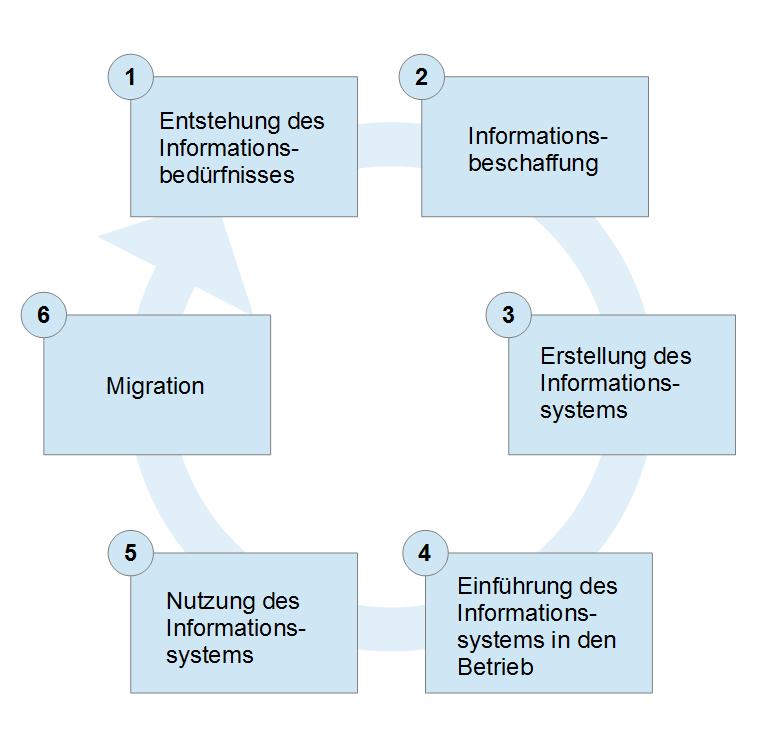
\includegraphics[width=10.851cm,height=10.608cm]{ErsteVersionderHausarbeit11Boris-img/ErsteVersionderHausarbeit11Boris-img001.png}
\end{figure}

\bigskip


\bigskip


\bigskip


\bigskip


\bigskip


\bigskip


\bigskip


\bigskip


\bigskip


\bigskip


\bigskip


\bigskip


\bigskip


\bigskip


\bigskip


\bigskip


\bigskip


\bigskip


\bigskip


\bigskip


\bigskip

{\sffamily\color{black}
\textrm{\ \ \ \ \ \ \ \ }Abb. 1: Informations-Lebenszyklus}


\bigskip


\bigskip


\bigskip


\bigskip


\bigskip


\bigskip


\bigskip


\bigskip


\bigskip


\bigskip

{\sffamily\color{black}
\textsuperscript{8 }Dippold, R.; Meier, A.; Schneider, W.; Schwinn, K.; Unternehmensweites Datenmanagement: Von der
Datenbankadministration bis zum Informationsmanagement (Zielorientiertes Business Computing); 4. überarbeitete und
erweiterte Auflage;2005; Vieweg-Verlag; Braunschweig, Wiesbaden }

{\sffamily\bfseries\color{black}
1.1.2 Informationsmanagementmodelle in der Literatur}

{\sffamily\color{black}
\newline
In der deutschsprachigen Literatur lassen sich viele verschiedene Arbeiten und Definitionen zum Thema
Informationsmanagement finden, die sich zum Teil deutlich voneinander unterscheiden. Im Folgenden wollen wir kurz auf
die Informationsmanagementmodelle- und Sichtweisen von Heinrichs, Wollnik und Krcmar eingehen.}


\bigskip


\bigskip

{\sffamily\color{black}
1.1.2.1 Informationsmanagement nach Heinrich\textsuperscript{9}}

{\sffamily\color{black}
\newline
Lange Zeit stellte das 1987 erschienene Werk von Lutz Heinrich das deutschsprachige Standardwerk im Bereich des
Informationsmanagement dar. Entsprechend wurde es auch als Lehrbuch an Hochschulen eingesetzt.\textsuperscript{10}}


\bigskip

{\sffamily
\textcolor{black}{Laut Heinrich wird unter Informationsmanagement das “Leitungshandeln (Management) im Unternehmen im
Bezug auf Information und Kommunikation” verstanden.}\textcolor{black}{\textsuperscript{9 \ }}\textcolor{black}{Es
umfasst alle Führungsaufgaben, die sich mit Information und Kommunikation befassen. Diese Informations- und
Kommunikationsaufgaben werden als Informationsfunktion bezeichnet, die den Schwerpunkt des Informationsmanagements
darstellt. Das Ziel des Informationsmanagements laut Heinrich ist es, eine Informationsinfrastruktur aufzubauen, die
die Verteilung, Produktion und Nutzung vom Informationen zur Aufgabe hat. Die Informationsinfrastruktur dient dazu, das
Leistungspotenzial der Informationsfunktion umzusetzen und somit einen optimaler Beitrag zum Unternehmenserfolg zu
leisten.}\textcolor{black}{\textsuperscript{10}}\textcolor{black}{ }}


\bigskip


\bigskip


\bigskip


\bigskip


\bigskip

{\sffamily\color{black}
\textcolor[rgb]{0.14509805,0.14509805,0.14509805}{\textsuperscript{9}}\textcolor[rgb]{0.14509805,0.14509805,0.14509805}{
Lutz J. Heinrich: }\textit{\textcolor[rgb]{0.14509805,0.14509805,0.14509805}{Informationsmanagement.
}}\textcolor[rgb]{0.14509805,0.14509805,0.14509805}{8. Auflage. Oldenbourg Wissenschaftsverlag, München/ Wien 2005} }

{\sffamily\color{black}
\textsuperscript{10} Vgl. Heinrich, Lutz; Informationsmanagement – Planung, Überwachung und Steuerung der
Informationsinfrastruktur; 7. Vollständig überarbeitete und ergänzte Auflage 2002, Oldenbourg-Verlag; München,
Wiesbaden }

{\sffamily\color{black}
Für die Umsetzung der Ziele werden die Aufgaben des Informationsmanagements in drei Ebenen strukturiert.}


\bigskip

\liststyleLi
\begin{itemize}
\item {\sffamily
\textcolor{black}{Die }\textbf{\textcolor{black}{strategische}}\textcolor{black}{ Ebene plant, überwacht und steuert die
Informationsinfrastruktur.}}
\item {\sffamily
\textcolor{black}{Die }\textbf{\textcolor{black}{administrative}}\textcolor{black}{ Ebene plant, überwacht und steuert
die Komponenten der Informationsinfrastruktur (z.B. Anwendungssysteme, Mitarbeiter, Bestand an Daten).}}
\item {\sffamily
\textcolor{black}{Die }\textbf{\textcolor{black}{operative}}\textcolor{black}{ Ebene umfasst Aufgaben und Nutzung der
Informationsinfrastruktur. Mögliche Aktionsfelder für die operative Aufgabenebene stellen den laufenden Betrieb, die
Nutzerunterstützung und die Störungsbeseitigung dar.}}


\bigskip
\end{itemize}
{\sffamily\color{black}
Auf jeder Aufgabenebene werden Methoden, Techniken und Werkzeuge eingesetzt, die die Durchführung der strategischen,
administrativen und operativen Aufgaben durchführt und unterstützt. Die Gesamtheit dieser Methoden und Techniken wird
von Heinrich als Information Engineering bezeichnet.}


\bigskip

{\sffamily
\newline
\textcolor{black}{1.1.2.2 Informationsmanagement nach Wollnik}\textcolor{black}{\textsuperscript{11}}}


\bigskip

{\sffamily\color{black}
Michael Wollnik gliedert das Informationsmanagement in drei Ebenen.\newline
}

{\sffamily
\textcolor{black}{Die }\textbf{\textcolor{black}{Ebene des Informationseinsatzes}}\textcolor{black}{ und dessen
Management befasst sich mit der Integration von Informationen in Produkte und Dienstleistungen. Des weiteren befasst es
sich mit der Erschließung neuer Märkte durch den Einsatz von Informationstechnologie.\newline
}}

{\sffamily
\textcolor{black}{Die }\textbf{\textcolor{black}{Ebene der Informations- und Kommunikationssysteme}}\textcolor{black}{
stellt die mittlere Managementebene dar. Laut Wollnik bestehen Informationssysteme aus folgenden Elementen/Komponenten:
Aufgaben, Informationen, Personen, Geräte, Organisation und Programme. Diese bestimmen die Struktur eines
Informationssystems. Die Aufgaben dieser Ebene sind die Festlegung, Erhaltung }\textcolor{black}{und Modifikation
dieser Strukturen während des Lebenszyklus des Informationssystems.}}

{\sffamily\color{black}
Ein weiteres Handlungsobjekt dieser Ebene sind die Prozesse zur Gestaltung von Informationssystemen, die geplant,
organisiert und kontrolliert werden müssen.}

{\sffamily\color{black}
Diese Ebene stellt das Verbindungsglied zwischen den betrieblichen Aufgaben (Ebene Eins) und der technischen
Infrastruktur (Ebene Drei) dar.}


\bigskip

{\sffamily
\textcolor{black}{Die }\textbf{\textcolor{black}{Ebene der Informations- und
Kommunikationsinfrastruktur}}\textcolor{black}{ ist die unterste der drei Ebenen und befasst sich mit der
Informationstechnologie. Dazu zählen laut Wollnik die Hard- und Software, aber auch die inhaltlichen Strukturen
(zentrale Informationsbestände, Zugriffsberechtigungen auf Informationen). Kernaufgabe dieser Ebene ist der Betrieb und
die Entwicklung der Infrastrukturen.}}


\bigskip

{\sffamily\color{black}
Diese drei Ebenen sind hierarchisch strukturiert und stellen den jeweils übergeordneten Ebenen Dienstleistungen zur
Verfügung bzw. stellen Anforderungen an die jeweils untergeordneten Ebenen.\newline
}



\begin{figure}
\centering
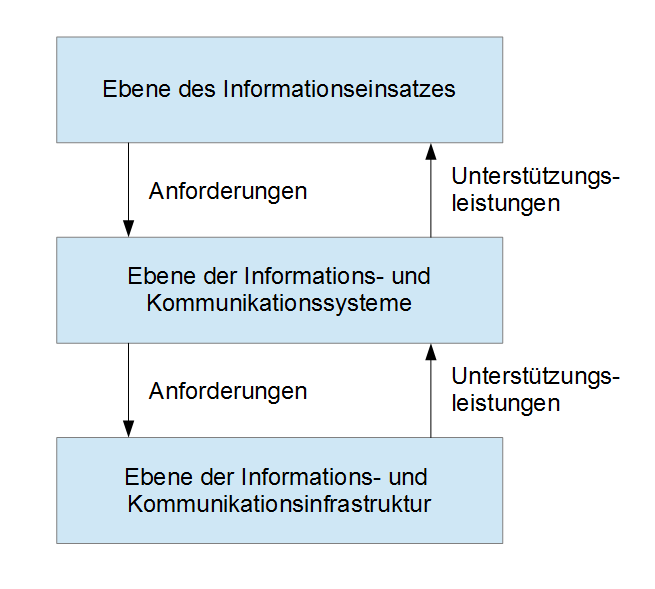
\includegraphics[width=9.301cm,height=8.303cm]{ErsteVersionderHausarbeit11Boris-img/ErsteVersionderHausarbeit11Boris-img002.png}
\end{figure}

\bigskip


\bigskip


\bigskip


\bigskip


\bigskip


\bigskip


\bigskip


\bigskip


\bigskip


\bigskip


\bigskip


\bigskip

{\centering\sffamily\color{black}
Abb. 2: Ebenenmodell nach Wollnik (Quelle: Wollnik (1988, S. 38)
\par}


\bigskip

{\sffamily\color{black}
Dieses einfache Ebenenmodell liefert auch die Grundlage für viele weitere Informationsmanagement- modelle, unter anderem
auch das von Krcmar.}


\bigskip

{\sffamily\color{black}
\textsuperscript{11 }Vgl. Wollnik, Michael; Ein Referenzmodell des Informations-Management in: Information Management 3;
1988 }

{\sffamily\color{black}
1.1.2.3 Informationsmanagement nach Krcmar\textsuperscript{12}\newline
}

{\sffamily\color{black}
Krcmars Strukturierung des Informationsmanagement basiert auf dem Ebenenmodell von Wollnik, erweitert es aber um
allgemeine Führungsaufgaben mit ebenenübergreifenden Funktionen (IT-Governance, Strategie, IT-Prozesse, IT-Personal,
IT-Controlling).}


\bigskip

{\sffamily\color{black}
Krcmar gliedert das Informationsmanagement in drei Teilbereiche:}


\bigskip

\liststyleLii
\begin{itemize}
\item {\sffamily
\textcolor{black}{Die }\textbf{\textcolor{black}{Informationswirtschaft}}\textcolor{black}{, die sich mit dem Angebot,
der Nachfrage und Verwendung von Informationen beschäftigt.}}
\item {\sffamily
\textcolor{black}{Die }\textbf{\textcolor{black}{Informationssysteme}}\textcolor{black}{, die das Management von Daten,
Prozessen und dem Anwendungslebenszyklus zur Aufgabe haben.}}
\item {\sffamily
\textcolor{black}{Die }\textbf{\textcolor{black}{Informations- und Kommunikationstechnik}}\textcolor{black}{, die die
Speicherung, Verarbeitung und Kommunikation von Information als Basisfunktionalitäten aufweist.}}


\bigskip
\end{itemize}
{\sffamily\color{black}
In Kapitel 1.2 wird genauer auf den Aufbau des Informationsmanagementmodells von Krcmar eingegangen.}

{\sffamily\color{black}
Da Krcmar mit seinen Publikationen zum Thema Informationsmanagement breiter aufgestellt ist als andere Autoren und er
entsprechend oft zitiert wird, soll er auch in dieser Arbeit als Quelle für die nachfolgenden Kapitel sein. }


\bigskip


\bigskip


\bigskip


\bigskip


\bigskip


\bigskip


\bigskip


\bigskip


\bigskip


\bigskip

{\sffamily\color{black}
\textsuperscript{12} Krcmar, Helmut: Informationsmanagement; 5. Auflage 2010; Springer-Verlag Berlin Heidelberg}

{\sffamily\bfseries\color{black}
1.1.3 Ziele des Informationsmanagements}


\bigskip

{\sffamily\color{black}
Das Informationsmanagement verfolgt zwei grundlegende Zielsetzungen. Das erste Ziel ist die Koordination der
Informationslogistik bzw. die Gewährleistung der adressatengerichteten Informationsversorgung. Das zweite Ziel ist die
Unterstützung der Unternehmensziele durch eine zielgerichtete und wirtschaftliche Steuerung der
Informatik.\textsuperscript{13} Die Aufgaben des Informationsmanagements leiten sich aus diesen Zielen ab und werden im
Kapitel 1.3 näher beleuchtet.}


\bigskip

{\sffamily\color{black}
1.1.3.1 Koordination der Informationslogistik}


\bigskip

{\sffamily\color{black}
In erster Linie ist das Ziel des Informationsmanagements, tatsächlich relevante Information von der Menge an verfügbaren
und eventuell unnützen Information zu trennen, die für einen Entscheidungsprozess benötigt werden. Hierzu muss jedoch
erst einmal ein Informationsbedarf vorliegen, der die Art, Menge und Beschaffenheit der Informationen bestimmt und auf
dessen Grundlage eine Entscheidung getroffen werden kann. Die Definition des Informationsbedarfs hängt einerseits vom
Entscheider, andererseits aber auch von den Anforderungen der zu treffenden Entscheidung ab.}


\bigskip

{\sffamily\color{black}
Der Informationsbedarf lässt sich grundsätzlich in zwei Kategorien einteilen: in den objektiven und den subjektiven
Informationsbedarf.\textsuperscript{14}}

{\sffamily
\textcolor{black}{Der }\textbf{\textcolor{black}{objektive }}\textcolor{black}{Informationsbedarf wird in erster Linie
durch die Entscheidung festgelegt und baut auf der Aufgabenbeschreibung des Entscheiders und den jeweiligen
Marktgegebenheiten auf.}}

{\sffamily
\textcolor{black}{Der }\textbf{\textcolor{black}{subjektive }}\textcolor{black}{Informationsbedarf wird primär durch den
Entscheider festgelegt. Welche Informationen für die Entscheidung relevant sind, werden durch die Einschätzungen und
Präferenzen des Entscheiders mitbestimmt.}}


\bigskip


\bigskip


\bigskip

{\sffamily\color{black}
\textsuperscript{13} Vgl. Zarbekow, Brenner 2004, S. 3-21}

{\sffamily\color{black}
\textsuperscript{14} Vgl. Picot et al. 2003, S. 81-82}

{\sffamily\color{black}
Aus der Überschneidung des objektiven und subjektiven Informationsbedarfs entsteht die Informationsnachfrage, die
wiederum maßgeblich vom Informationsangebot abhängt. Somit legt der Informationsbedarf}


\bigskip

\liststyleLiii
\begin{itemize}
\item {\sffamily\color{black}
die Beschaffenheit (Qualität)}
\item {\sffamily\color{black}
den Zeitpunkt der Lieferung}
\item {\sffamily\color{black}
den Ort, an dem geliefert wird }
\item {\sffamily\color{black}
das Medium, über das geliefert wird}
\end{itemize}

\bigskip

{\sffamily\color{black}
der Information fest. Im Hinblick auf die Unternehmensziele sollten die Informationen als Ressource angesehen
werden.\textsuperscript{15} }


\bigskip

{\sffamily\color{black}
1.1.3.2 Informationsmanagement als Unterstützung der Unternehmensziele\newline
}

{\sffamily\color{black}
Das Informationsmanagement bildet einen Teil der Unternehmensführung ab, der die wirtschaftliche Steuerung der
Informatik (d.h. Mitarbeiter, Prozesse, organisatorische Teilbereiche und die eingesetzten Informationstechnologien)
zur Verantwortung hat. Die Rahmenbedingungen für die Informationslogistik werden so gestaltet, dass diese Informatik
und deren Leistungen auf die Unternehmensziele ausgerichtet ist.\textsuperscript{16} Dazu sollte eine geeignete und
zweckorientierte Informationsinfrastruktur (Systemdenken, Rationalisierung, Orientierung am Beschaffungs- und
Absatzmarkt) bereitgestellt werden.\textsuperscript{17}}


\bigskip


\bigskip


\bigskip


\bigskip


\bigskip


\bigskip

{\sffamily\bfseries\color{black}
\textmd{\textsuperscript{15 }}\textrm{\textmd{Vgl. u.a. Bode, J.: Der Informationsbegriff in der
Betriebswirtschaftslehre In: Zfbf.; Bd. 49 S. 449 – 469; 1997; Verlagsgruppe Handelsblatt, Düsseldorf}} }

{\sffamily\bfseries\color{black}
\textmd{16 \ Voß, Gutenschwager 2001, S65-68}}

{\sffamily\color{black}
\textsuperscript{17 }\textrm{Vgl. u.a. Vieweger, Bernd; Informationsmanagement;} 2013}

{\sffamily\bfseries\color{black}
Quellenverweise:}

{\sffamily\color{black}
Voß, Stefan; Gutenschwager, Kai: Informationsmanagement. Springer: Berlin et al., 2001}


\bigskip

{\sffamily\color{black}
Wittmann, W.: Unternehmung und unvollkommene Information. Köln, Opladen: Westdeutscher, 1959}


\bigskip

{\sffamily\color{black}
Dr. Lüpke, Michael, Gerlingen \url{http://www.dr-luepke.de/Seiten/InfoMangmt1.htm}, Stand: 2010}


\bigskip

{\sffamily\color{black}
Probst, Gilbert J. B.; Raub, Steffen; Romhardt, Kai; Wissen managen; 5. Auflage 2006; Gabler-Verlag; Wiesbaden}


\bigskip

{\sffamily\color{black}
Bode, J.: Der Informationsbegriff in der Betriebswirtschaftslehre In: Zfbf.; Bd. 49; 1997; Verlagsgruppe Handelsblatt,
Düsseldorf}


\bigskip

{\sffamily\color{black}
Teubner, A.: Information als Wirtschaftsgut und Produktionsfaktor; In: WISU, Bd. 34; 2005 }


\bigskip

{\sffamily\color{black}
Krcmar, Helmut: Informationsmanagement; 5. Auflage 2010; Springer-Verlag Berlin Heidelberg}


\bigskip

{\sffamily\color{black}
Dippold, R.; Meier, A.; Schneider, W.; Schwinn, K.; Unternehmensweites Datenmanagement: Von der Datenbankadministration
bis zum Informationsmanagement (Zielorientiertes Business Computing); 4. überarbeitete und erweiterte Auflage;2005;
Vieweg-Verlag; Braunschweig, Wiesbaden }


\bigskip

{\sffamily\color{black}
Heinrich, Lutz; Informationsmanagement – Planung, Überwachung und Steuerung der Informationsinfrastruktur; 7.
Vollständig überarbeitete und ergänzte Auflage 2002, Oldenbourg-Verlag; München, Wiesbaden }


\bigskip

{\sffamily\color{black}
\textcolor[rgb]{0.14509805,0.14509805,0.14509805}{Lutz J. Heinrich:
}\textit{\textcolor[rgb]{0.14509805,0.14509805,0.14509805}{Informationsmanagement.
}}\textcolor[rgb]{0.14509805,0.14509805,0.14509805}{8. Auflage. Oldenbourg Wissenschaftsverlag, München/ Wien 2005} }


\bigskip

{\sffamily\color{black}
Wollnik, Michael; Ein Referenzmodell des Informations-Management in: Information Management 3; 1988 }

{\sffamily\color{black}
Zarnekow, Rüdiger; Brenner, Walter: Integriertes Informationsmanagement: Vom Plan, Built, Run zum Source, Make, Deliver.
In: Zarnekow, Rüdiger; Brenner, Walter; Grohmann, Helmut H. (Hrsg.): Informationsmanagement – Konzepte und Strategien
für die Praxis. dpunkt: Heidelberg, 2004}


\bigskip

{\sffamily\color{black}
Picot, Arnold; Reichwald, Ralf; Wigand, Rolf: Die grenzenlose Unternehmung. 5. Aufl., Gabler: Wiesbaden 2003}


\bigskip
\end{document}
